In the world there is no natural source of parallel beams. Each beam of light can be considered originating from a simple origin: point light source, which emits anisotropic light in all directions. Thus a normal light source cannot provide perfect focused beams for optical applications. TEM$_{00}$ mode of a laser source is a perfect plane wave with Gaussian transverse irradiance profile\cite{CVI_Melles_Griot_Technical_Guide}. Therefore the laser light is considered as a beam propagating in a well-defined direction with limited spreading in transversal dimensions.\\ 
In \cite{ script_FT_TET} the transversal e-field components of Gaussian beam is assumed as (\ref{eq:gaussian_01}).
\begin{equation}
E_{x}=\psi(x,y,z)e^{-jk_{0}nz}
\label{eq:gaussian_01}
\end{equation}
We insert (\ref{eq:gaussian_01}) into wave equation (\ref{eq:wave_equation})
\begin{equation}
\bigtriangleup E_{x}+k^{2}_{0}n^{2}E_{x}=0
\label{eq:wave_equation}
\end{equation}
 and obtain partial differential form (\ref{eq:gaussian_02}). Because the paraxial beams spread slowly in transversal direction due to the z-axis, the term $\frac{\partial ^{2}\psi}{\partial z^2}$ is very smaller than other terms. Thus equation (\ref{eq:gaussian_02}) become an approximation (\ref{eq:gaussian_03}).
\begin{equation}
\frac{\partial ^{2}\psi}{\partial x^2}+\frac{\partial ^{2}\psi}{\partial y^2}+\frac{ \partial ^{2}\psi}{\partial z^2}-2jk_{0}n\frac{\partial\psi}{\partial z}=0
\label{eq:gaussian_02}
\end{equation}
\begin{equation}
\frac{ \partial ^{2}\psi}{\partial x^2}+\frac{\partial ^{2}\psi}{\partial y^2}-2jk_{0}n\frac{\partial\psi}{\partial z}=0
\label{eq:gaussian_03}
\end{equation}
The equation(\ref{eq:gaussian_03}) can also be transformed into cylinder coordinate and become (\ref{eq:gaussian_04})
\begin{equation}
\frac{1}{r}\frac{\partial}{\partial r}\left(r\frac{\partial z}{\partial r}\right)+\frac{1}{r^2}\frac{ \partial ^{2}\psi}{\partial \phi^2}-2jk_{0}n\frac{\partial\psi}{\partial z}=0
\label{eq:gaussian_04}
\end{equation}
(\ref{eq:gaussian_05}) is one general solution of (\ref{eq:gaussian_04})
\begin{equation}
\psi(r,z)=\psi_{0}\exp\left(-j\left[P(z)+2 \frac{ k_{0}n}{2q(z)}r^2\right]\right)
\label{eq:gaussian_05}
\end{equation}
Where $P(z)$ and $q(z)$ meet the equation (\ref{eq:gaussian_04}) for any $r$. The term $q(z)$ has also the relation(\ref{eq:gaussian_06}) with some physical variables $w(z)$ and $R(z)$
\begin{equation}
\frac{1}{q(z)}=\frac{1}{R(z)}-\frac{j\lambda}{\pi nw^{2}(z)}
\label{eq:gaussian_06}
\end{equation}
Where $w(z)$ is the $1/e^2$ irradiance radius due to propagating distance z and $R(z)$ is the wavefront radius of curvature due to propagating distance z
\begin{equation}
w(z)=w_{0}\sqrt{1+\left(\frac{\lambda z}{n\pi w^{2}_{0}}\right)^{2}}
\label{eq:gaussian_07}
\end{equation}
\begin{equation}
R(z)=z\left[1+\left(\frac{\lambda z}{n\pi w^{2}_{0}}\right)^{2}\right]
\label{eq:gaussian_08}
\end{equation}

If (\ref{eq:gaussian_06}) is inserted in (\ref{eq:gaussian_05}) then we can obtain a Gauss form result 
\begin{equation}
\psi(r,z)=w_{0}\exp\left(-\frac{r^2}{w^2_{0}}\right) \text{.}
\label{eq:gaussian_09}
\end{equation}
That means the field of a Gaussian beam is in transversal dimensions a Gaussian distribution like Fig. \ref{fig:gaussian_verteilung}.\\

\begin{figure}[!ht]
\centering
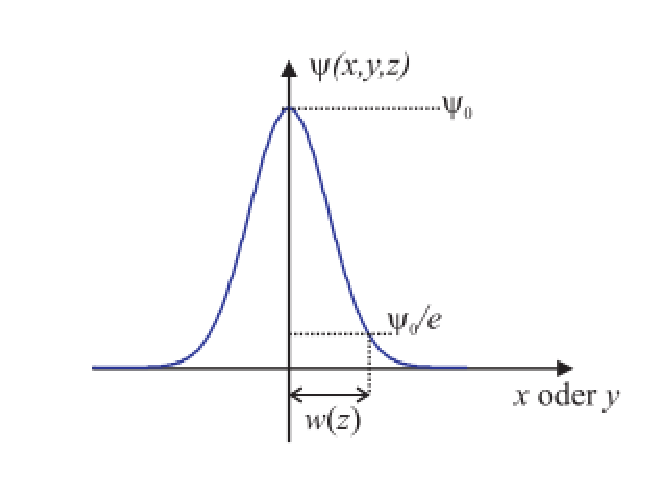
\includegraphics[width=0.6\textwidth]{bilder/gussian_verteilung}
\caption{Transversal profile of the Gaussian beam is the curve of Gaussian functions. At the beam center the field has the maximum value. At the distance of $w(z)$ form the center the field decline to $1/e$ of the peak value.}
\label{fig:gaussian_verteilung}
\end{figure}
According to definitions of $w(z)$ and $R(z)$ in (\ref{eq:gaussian_07}-\ref{eq:gaussian_08}) the longitudinal profile of Gaussian beams can be drawn as Fig. \ref{fig:gussian_profile}.
\begin{figure}[!ht]
\centering
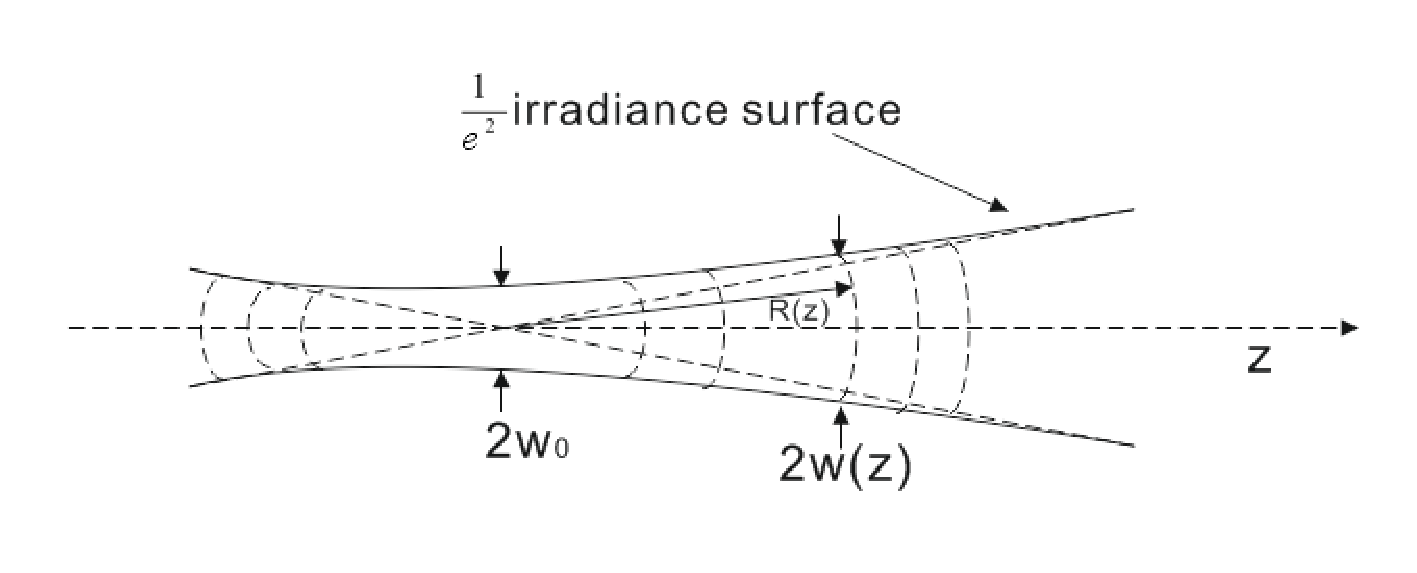
\includegraphics[width=0.9\textwidth]{bilder/gussian_profile}
\caption{The lateral profile of Gaussian beams presents the domain of beam power from peak value to $1/e^2$ peak value. $w(z)$ represents the radius of this profile. $R(z)$ is the radius of wavefronts.}
\label{fig:gussian_profile}
\end{figure}
From the beam axis to the distance of beam radius $w(z)$ the intensity drops to $1/e^{2} (\sim13.5\%)$ of the maximum value. That means, a hard aperture with radius $w$ can transmit $\sim86.5\%$ of the optical power.

%Spot Size
\subsubsection*{Spot Size}
Another important characteristic of Gaussian beams is Spot Size. In a cross-section of a Gaussian beam the beam intensity is approximately distributed as Gaussian function. The spot size is the diameter of the domain at whose edge the value of the electrical field intensity decays to $1/e$ of the peak value, otherwise the energy density decays to $1/e^2$ of the peak value.
